\documentclass[12pt,a4paper]{article}
\usepackage[utf8]{inputenc}
\usepackage[english]{babel}
\usepackage{url}
\usepackage{hyperref}
\usepackage{amsmath}
\usepackage{amsfonts}
\usepackage{amssymb}
\usepackage{graphicx}
\usepackage{float}
\usepackage{lipsum}
\usepackage{multicol}
\usepackage{xcolor}
\usepackage{caption}
\usepackage{capt-of}
\usepackage{textcomp}
\usepackage[inline]{enumitem}
\captionsetup[figure]{skip=2pt}
\usepackage{booktabs}
\usepackage[
    backend=biber,
    style=apa,
    citestyle=numeric,
    sorting=nyt,
    labelnumber=true
]{biblatex}
\defbibenvironment{bibliography}
  {\list
     {\printtext[labelnumberwidth]{
        \mkbibbrackets{\printfield{labelnumber}}}}
     {\setlength{\labelwidth}{\labelnumberwidth}
      \setlength{\leftmargin}{\labelwidth}
      \setlength{\labelsep}{\biblabelsep}
      \addtolength{\leftmargin}{\labelsep}
      \setlength{\itemsep}{\bibitemsep}
      \setlength{\parsep}{\bibparsep}}
      \renewcommand*{\makelabel}[1]{##1\hss}}
  {\endlist}
  {\item}
\addbibresource{sources.bib}
\newcommand{\celda}[1]{
	\begin{minipage}{2.5cm}
		\vspace{5mm}
		#1
		\vspace{5mm}
	\end{minipage}
}
\definecolor{azul}{rgb}{0.0, 0.53, 0.74}
\definecolor{darkred}{rgb}{0.7, 0.2, 0.32}
\usepackage[left=2.00cm, right=2.00cm, top=2.00cm, bottom=2.00cm]{geometry}
\author{Dalia Muth}
\title{Bachelor Thesis}

\begin{document}

    \begin{center}
    \thispagestyle{empty}
    \vspace*{3cm}
    \LARGE{University of Osnabrück}\\[0.25ex]
    \LARGE{Institute of Cognitive Science}\\[1.5ex]
    \large{Department of Neuroinformatics}\\
    \vspace*{0.3cm}
    \vspace*{2cm}
    %\textbf{\LARGE{Bachelor Thesis}}
    \medskip\par
    %\textbf{\normalsize{submitted for the degree of}} \\[2ex]
    \Large{Bachelor Thesis}\\
    \vspace*{1.5cm}
    \Large{\textbf{Noise-Induced Synchrony and the Effects on Spike Pattern Length in a Spiking Neural Network}}\\
    \vspace*{1.5cm}
    %\large{Lorem ipsum dolor sit amet, consectetur adipiscing elit}\\[-1.5ex]
    \bigskip\par
    \large{Dalia Muth}\\[0.5ex]
    \large{Matriculation Nr.: 1005371}\\ [5ex]
    \vspace*{2cm}
    \\[1ex]
    \large{Submission Date:  & 6th April 2026}\\[0.5ex]
    \large{Supervisors: & MSc. Viktoriia Zemliak, Prof. Gordon Pipa}\\ [5ex]
    \end{center}

    \newpage
    \tableofcontents
	
    \newpage
	\begin{figure}[H]
		\raggedright
	\end{figure}

	\vspace{7.5mm}
	
	\begin{center}
		{\Large \textbf{Noise-Induced Synchrony and the Effects on Spike Pattern Length in a Spiking Neural Network}}\\
		\vspace{2mm}
		{\large Dalia Muth$^{1}$}\\
		\vspace{7.5mm}
		$^1$\textit{Osnabrück University, Institute of Cognitive Science, Department for Neuroinformatics} \\
	\end{center}

	\begin{center}
		\textcolor{darkred}{\rule{150mm}{0.5mm}}
	\end{center}		

	\begin{abstract}
		The underlying coding mechanims for information processing in the brain are of high relevance in biological and technical research. Two main electrical coding schemes have been identified in neurons, rate code and temporal code. Rate code has received most attention in previous research due to its strong and easily identifiable event-correlation results. In recent years, temporal code has regained interest, specifically on the topic of synchrony. Advantages of synchrony code include increased temporal precision, shorter timescales, signal processing of distributed information, and enhanced signal summation. The impact of synchrony code can be demonstrated by analyzing spike pattern lengths in a laterally connected spiking neural network. Increased synchrony is expected to shorten spike pattern length due to parallelization of processes. In this experiment, the effects of noise-induced synchrony on spike pattern length in a spiking neural network were evaluated. The model consisted of a single recurrent layer representing a small laterally connected neuron cluster. Synchrony was found to emerge from an optimal non-zero amount of noise and to decrease spike pattern length, enabling efficient information processing for distributed signals.
		\vspace{2mm}
	\end{abstract}

	\begin{center}
		\textcolor{darkred}{\rule{150mm}{0.5mm}}
	\end{center}		

	\vspace{5mm}

    
	
	\begin{multicols}{2}

        \section{Introduction}
			With the ambition to better understand how a complex system like the human brain coordinates around 86 billion processing units \cite{U}, performing an estimate of 6000 thoughts per day \cite{T}, neural coding mechanisms are extensively studied. Previous work has revealed detailed insights on the physical structure of the brain, as well as lower order mechanisms, but understanding how neural mechanisms lead to the thoughts we experience remains a challenge \cite{R}. Different types of neural coding mechanisms have been detected and researched, with the focus on rate code, because of its consistency in results and easy detectability \cite{X, R, L}. Rate-based code conveys information by relating the average pre-synaptic firing frequency to a post-synaptic output. Research on other forms of neural coding is still sparse, because rate code has proven to be reliable, comprehensible, reproducible and robust in its results \cite{X}. Temporal code has received less attention in previous research due to difficulties in simultaneously recording the activity of multiple neurons, and major doubts about its relevance. Specifically synchrony code, a sub-type of temporal code, has received strong criticism. Neural synchrony can be described as the firing of different neurons at the same time or with a consistent, coordinated offset. Recordings of neural synchrony in experimental research are abundant, however, the phenomenon has commonly been reduced to a mere by-product, disregarding its potential as a coding mechanism \cite{M, L, G}. Despite the challenges, synchrony code has recently regained interest.
            
        \subsection{Synchrony Code}
            Synchrony code is a type of temporal coding that works through a mechanism called \textit{coincidence detection}, which attributes value to correlations between spike timings of different neurons. Synchrony code poses promising theoretical advantages \cite{R}.
            
            In comparison to rate code, synchrony code cannot be evaluated on the basis of singular neurons, but relies on multicell analysis, i.e. the recording and evaluation of different spiking neurons simultaneuously \cite{G}. This creates the opportunity to relate spatially distributed signals to coherent patterns of functional importance. It may serve to solve the binding problem that rate code faces, which refers to the challenge of relating signal processing on a small unit level to complex thoughts. Rate code struggles to solve this issue, due to it being limited to local operations, whereas synchrony code is able to process signals distributed across the network \cite{G, R}.
            
            Spatial distribution of related signals drastically increases the overall impact of information exchange on the whole neuronal system: With rate code operating on a singular cell level, one information unit is unable to influence the whole system when its information changes, due to longer pathways between individual neurons. In contrast, if information is encoded in multiple, spatially distributed cells, overall impact is increased through shorter pathways and combined activations. This enables encoding and decoding at a higher grain of neuronal representation, but also allows for more efficient code forwarding due to spatially distributed, parallel processing \cite{R, L}.
            
            Not only does synchrony code lead to increased efficiency by greater spatial coverage, it can also operate on very fast timescales. Rate code relies on temporal summation, which works on timescales with the same order of magnitude as the average interspike interval (ISI) \cite{R, Z}. Coincidence detection on the other hand can process information on a few millisecond timescale, which is often only a fraction of the average ISI \cite{R}. This leads to a substantial increase in processing speed. A further increase in efficiency that can be achieved with synchrony code, is related to the nature of synchronized spikes, which is the increase in saliency of signals through spatial summation and backpropagating dendrites \cite{G}: For the same amount of absolute spikes, a stronger and more immediate response can be evoked from synchronous spatial summation compared to temporal summation. If pre-synaptic spikes only reach the synapse in temporal summation, a the post-synaptic output will be delayed in time compared to the same amount of input arriving in the form of spatial summation. Furthermore, in the case of low spike frequency of solely temporally summing signals, the neuron's voltage may remain below the threshold entirely \cite{G, Z}. 
            
            In summary, synchrony code allows for increased efficiency at a temporal and spatial level, which further allows for important metabolic advantages \cite{L}. With the many benefits of synchrony coding, it would be highly unlikely that the nervous system and the brain do not harness it at all. Nonetheless, temporal code does not come without downsides, which is why most of recent research suggests a combination of rate code, synchrony code, and other potential coding schemes to be the most plausible and efficient \cite{L, G, R}.
        
        \subsection{Neural Noise}
            Neural noise is a result of the neuronal network complexity on a molecular level. Ion channel activity, protein production and decomposition, as well as synaptic input artifacts are non-deterministic processes that cause irregular membrane voltage fluctuations \cite{Q}. In contrast to prior beliefs, recent studies have shown that neural noise is not merely random occurence that the system is built to work around, but that it may be of functional biological relevance \cite{Q, P, O}. Furthermore, neural noise was found to support or cause the emergence of synchrony, due to a process called stochastic resonance \cite{B, P, Q}. Stochastic resonance can occur if neurons receive an oscillatory drive as well as a non-zero amount of noise, which induces synchrony by shifting the activity phases of the different involved neurons. It was also found that in non-linear systems, similar behavior can be induced absent of a continuous external oscillatory drive. In that case, increased noise amplitude decreases the variation coefficient, leading to an increase in spike correlations. This phenomenon is referred to as \textit{coherence resonance} \cite{O, P, Q}.
            
        \subsection{Synchrony in Dynamical Systems Theory}
            Another perspective in favor of investigating noise effects on synchrony is the research on modeling the brain as a complex dynamical system. \textcite{W} suggests that the brain possesses key attributes of complex dynamical systems, specifically immense complexity and sensitivity to small changes. Dynamical systems theory offers a potential solution to the question of how small changes on the molecular level could lead to big overall changes manifesting in cognitive states. If we assume the brain to be a complex dynamical system, single-cell activity becomes much less relevant than multi-cell coding. This results form the fact that the functioning of a complex dynamical system heavily relies on its ability to perform global transitions. In the brain as a dynamical system, such transitions would be carried out by neuronal activity, with synchrony as a promising candidate to initiate them \cite{W}. \textcite{Y} argues that noise is a relevant component in modeling the brain as a complex dynamical system. He distinguishes between dendritic and synaptic noise, the former defined as spontaneous emissions which may influence sub-threshold behavior, but too weak to activate a postsynaptic spike. The latter is described as stimulus-induced noise, potentially resulting in post-synaptic spikes. \textcite{Y} also refers to the theory that despite its chaotic behavior, noise may have the potential to induce order in a dynamical system.
        
        \subsection{Hypothesis}
            This paper aims to provide further insights into the effect of synchrony on temporal efficiency and its relevance as a coding mechanism. In addition, the experiment is supposed to demonstrate that the emergence of synchrony does not necessarily rely on preceding synchronized input.

            The proposed hypothesis is that 
            \begin{enumerate*}[label=(\arabic*)]
                \item\label{hyp1} noise alone can induce synchrony in a laterally connected spiking neural network and
                \item\label{hyp2} this synchrony is able to shorten spike pattern length in a spiking neural network. 
            \end{enumerate*}
            The proposed underlying mechanism is the parallelization of processes. If a laterally connected network ensemble is activated by one spike, the network it is expected to run through its connectivity patterns one step at a time. Whereas the same pattern induced simultaneously at different points of the network will be carried out in parallel, with decreased runtime. Consequently, the overall pattern length is shortened, allowing for increased temporal efficiency.


        \section{Related Work}
            Theoretical arguments for the interest in synchrony code were laid out in the introduction, however, experimental evidence on biological plausibility is crucial to justify further scientific investigation. The main criticism research on synchrony code receives is the possibility of it being an epiphenomenon without any efficacy \cite{G}. To counter this criticism, new research has to prove the functional importance of synchrony. This can be achieved by providing evidence of synchrony correlating with behavior, independent of modulations in firing rate.
            Different in vivo experiments have shown the functional role of synchrony in attention and arousal states, cognitive tasks, perception, expectancy and sensory mechanisms \cite{G}.
            
            Synchrony has shown to be of functional significance across different sensory domains. Olfactory pathways in locusts were found to harness synchrony as a coding scheme for odor distinction. When synchrony was disrupted, odor selectivity in some neurons decreased and hence their discrimination ability was impaired \cite{ZL}. A similar experiment of bees with additional behavioral testing confirmed their hypothesis that oscillatory synchronization in neurons at an early processing stage of the olfactory pathway codes for odor specificity. When synchronization of those neurons was inhibited, neurons that were activated later in the chain did not receive the input they needed for discrimination. Most importantly, these results were observed without significant changes in the firing rate of desynchronized neurons, concluding functional importance of synchrony \cite{ZM}.
            
            Evidence for the role of synchrony in perception comes from a study of cats with strabismic amblyopia. This is a condition where in order to avoid double vision, one eye becomes the dominant source for visual information, and the other eye develops perceptual deficits due to reduced usage. Synchrony patterns of neuron pairs, each corresponding to one of the eyes, were compared. It was found that neuron pairs connected to the normal eye showed significantly higher synchronization than pairs of the non-dominant eye. The observed effect was even stronger when cats were shown stimuli of different gratings, namely a coarse grating that could be identified reliably with both eyes, and a fine grating that was perceptible only with the normally functioning eye. For the normal eye, with finer gratings the response amplitude of neurons decreased, while synchronization remained stable. For the amblyopic eye, response amplitude as well as synchrony decreased. These results underline predictions that conditions where the amblyopic eye is at an even stronger disadvantage lead to even weaker synchronization. It has to be emphasized that the change in synchrony was not accompanied by firing rate modulations, which suggests that decreased synchronization is functionally correlated with impaired perception \cite{ZA}.
            
            A similar study investigated cats with interocular rivalry, a condition where one eye acts dominant over the other at every point in time. Here, dominance switches between eyes, but one eye usually favored. The cats were shown either congruent stimuli, where both eyes were presented with the same image, or incongruent stimuli, where each eye received a different image. For the incongruent condition, synchrony in neuron pairs corresponding to the dominant eye increased, while synchrony in neurons of the non-dominant eye decreased. In addition to synchrony, firing rates of those same neurons were analyzed and displayed no significant changes when switching from the congruent to the incongruent stimulus. These findings of significant reduction in synchrony for the perceptually impaired eye, independently of firing rate, support the theory that synchrony code is used for perceptual processing in the brain. Results may also imply a role of synchrony in attentional mechanisms \cite{ZB}.

            The role of synchrony was also investigated in the somatosensory and motor cortex. Synchronization was found to be greater in exploratory and self-organized movement tasks, rather than constrained and directed tasks \cite{ZC}. A specific correlation to movement execution was not found so far; synchrony was associated with the movement preparation period or anticipation, but was found to dissolve right before the onset of movement \cite{ZC, ZE, ZF}. Importantly, emergence of synchrony in the movement anticipation period was independent of firing rate changes \cite{ZE}. These findings suggest that synchrony is not necessarily used to code for actual movement execution. They rather support hypotheses of synchrony as a code for cognition, specifically perception and attention processes, such as binding of perceptual features or the mental separation of foreground and background \cite{ZC, ZE, ZF}. \textcite{ZF} derive a potential feature binding mechanism from their results, showing that most synchronized neuron pairs in their experiment had the same stimulus preference. \textcite{ZC} proposed that an attentional mechanism could be carried out through synchrony code by simultaneously pushing neurons that are attending to the same stimulus closer to the firing threshold.

            Further evidence for the importance of synchrony in cognitive processes can be derived when looking at the brain structures where it is found. Higher order cortical areas show increased synchrony compared to lower-order cortical areas \cite{L, G}. This synchrony gradient correlates with the degree of lateral interconnectivity, where the more strongly interconnected, higher order cortical areas appear to utilize synchrony code more often.
            Lower-order cortical areas, which are less densely laterally connected, are presumed to mostly harness rate code. This makes sense considering the nature of synchrony code, which is reliant on strong internal communication for coordination of spike times. Rate code in contrast is more effective in detecting feedforward drive, as it cannot interpret distributed information \cite{L}. These findings are in line with the observations that synchrony connects behaviorally to attention and perception, with main processing stages of these taking place in higher order cortical areas \cite{G}.
            While in vivo experiments are necessary to prove biological plausibility, studying the theoretical potentials of synchrony code in computational models is another crucial field of research. Modelling synchroy has revealed the potential of it to provide a mechanism that can store familiarity and memory information, where the structure of connectivity in a neuronal network can represent known patterns \cite{L, M}. Memory by synchrony operates through Hebbian plasticity, a long-term potentiation mechanism where neurons that fire together repeatedly strengthen their connections \cite{A, L}. Experiments like these not only enable future research to form hypotheses of potential biological mechanisms to then be tested in vivo, they also support technological progress and thus stay highly relevant.
            
            In summary, in vivo experiments on the one hand have gathered evidence for the functional role of synchrony in several sensory processing areas and for cognitive functions. More specifically, the type of cognitive fucntions that harness synchrony include perception, attention and grouping of stimuli. On the other hand, experiments that analyze synchrony in computational models support this process and provide valuable insights about this coding scheme from a different angle.

    
		\section{The Model}
        \subsection{Layer Setup and Recurrency}
			To examine how sub-threshold noise induces and affects synchrony, a spiking neural network (SNN) model was set up with a single recurrent layer. Recurrent layers as well as spiking neurons are not the standard procedure in current Artificial Neural Network (ANN) research, which SNNs are a sub-type of \cite{AA, AB}. Many ANN architectures rely on non-recurrent feedforward layers and the majority of artificial neurons utilize differentiable activation functions at their synapses, which allows for comparably simple backpropagation \cite{A}. Recurrent ANN layers are commonly used for sequential learning that integrate past input into the next step, however, randomly interconnected singular layers as in this model are uncommon. The recurrent layer in this model mimics a very simple patch of lateral connections with a certain connectivity probability, which is a structure shown to facilitate synchrony. The mechanism enabling synchrony in such networks is the recurring communication among neurons, leading to a self-organized adaptation to each other’s patterns through cross-activation \cite{L, AC}. The choice of one singular layer over multiple connected recurrent layers, as would be more biologically plausible, was made to keep results and evaluation simplistic and to reduce computational load to a minimum.In order to study the noise effect on synchrony isolated from other input current factors, this network was neither equipped with a learning algorithm, nor did it receive a task.
            
        \subsection{The Artificial Neuron}           
            Neurons with differentiable activation functions have mathematical advantages: due to their comparably simple derivatives, backpropagation using gradient descent, which is the current dominating learning algorithm for ANNs, can easily be implemented \cite{A, AD}. Spiking neural networks use a different type of integration at the synapse, where inputs sum up as binary input weights and create binary outputs. This makes backpropagation more analytically challenging \cite{AJ}. The binary outputs of artificial spiking neurons reflect more closely, but not completely, how biological neurons integrate. Very simply put, they communicate with the generation of a spike or no spike resulting from spike inputs. In biological neurons this is mediated by another complex, partially continuous process \cite{A}, but in SNNs a simpler mathematical formula is used. Neuronal integration in this paper was computed with the Leaky-Integrate-and-Fire (LIF) neuron (see Section ~\ref{sec:LIF}). The formula is a comparably simple analytical application of membrane time constant, firing threshold and refractory period, on an abstract level similar to the mechanism observed in biological neurons \cite{E}.
            
        \subsection{Connectivity}
            Working with only one recurrent layer, a singular connectivity matrix of the shape \verb+[to_neurons,from_neurons]+ was set up, with zero-values representing no connections and weights inserted for connecting neurons. The matrix was initialized with zeros and can be filled either manually or with a function automatically setting random connections at a connectivity percentage of choice. A \verb+auto_connect+ function was built to balance connections. This means that the funtion ensures each neuron is connected to a similar number of neurons and gets a similar amount of inputs at full activation. This builds a network structure where all neurons are interconnected rather than forming separated sub-networks. Unbalanced connections would likely decrease synchrony, since optimal adaptation to other neurons relies on short pathway feedback loops. With a balanced approach like in this model, each neuron is connected to other neurons in the network by few connections, facilitating quick communication. With the random connections a seed was used for reproducibility.
            
            Additionally an input matrix was set up with \verb+[neurons, time_steps]+, in case poisson inputs are supposed to be added. At default mode the input matrix is set to zeros.
            
            For analytical simplicity, the weights of the model were kept exclusively excitatory. Although some previous work has suggested that a balance of excitatory and inhibitory connections is favorable when trying to achieve synchrony, other recent studies have shown that inhibitory connections are not a hard requirement for synchrony \cite{M}.

        \subsection{Voltage Input}
            In modeling spiking neural networks, it is common practice to simulate input from another connected neuron population or randomly drawn from a poisson distribution, to mimic input as it is observed in biological neuron populations \cite{F, M, O}. For this model the spike input matrix was set up exclusively as an option to test code functionality and to support debugging processes. In the main experiment, input to neurons was given solely in the form of noise and lateral connections. The purpose of refraining from additional input was to isolate the noise effect, in order to test the experimental hypothesis.
            
        \subsection{Integration}
            In the integration step of the code, the neuron voltages are updated with the LIF calculation. The formula takes input currents and noise of the previous time step and calculates a membrane voltage update. The function then checks for a refractory period, where for all cases that are not in refractory, membrane voltage is compared to the threshold voltage and then updated. In the case that the neuron spiked after the voltage update, the last step is to reset the membrane voltage to the resting potential. Each of these steps is performed along the full neuron vector for one time step at the same time, because vector calculations are highly computationally efficient compared to loops. Code from \textcite{L} was used as a template to build this structure and adapted according to the simplified experimental use case. In the LIF formula (see Section ~\ref{sec:LIF}), voltage calculations modified by input currents are divided by the product of delta time and membrane time constant. Delta time represents the step size operated on, here set to 1 ms steps for simplicity. Analytically, the membrane time constant is the product of membrane capacitance and membrane resistance, which describes the rate at which the membrane rises or falls in biological neurons. The membrane time constant was set to 10, which lies within the biological range \cite{S}.
            
        \subsection{Simulation}
            The \textit{simulate} function was built to run through each time step of the spiking neural network simulation. Voltage and spikes are recorded in separate matrices after each integration time step. The integration function inside the time steps loop is fed with a matrix of external and lateral input currents, combined by a dot product. External input represents potential input streams from outside of the network, which was set to zero in the final experiment of this paper. Lateral input stems from the directed neuron connections inside the network. These inputs remain zero for connections where preceding neurons did not fire in the previous time step and are larger than zero for connections where preceding neurons did fire. Noise is added inside the integration function instead of combined into the input current matrix (Figure ~\ref{diagram}).

            \begin{figure}[H]
                \centering
                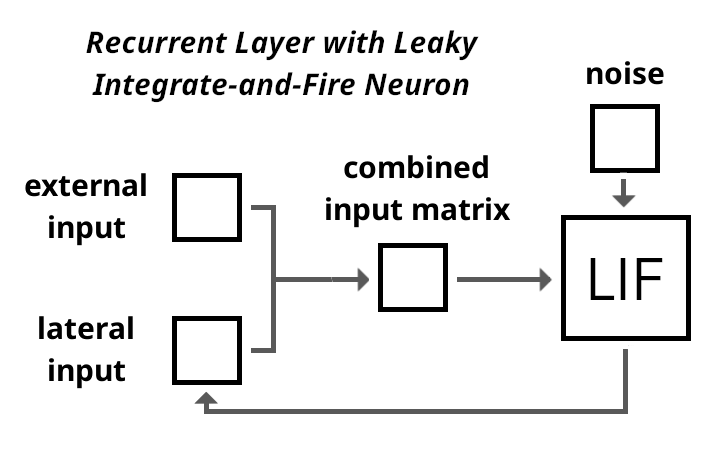
\includegraphics[width=\linewidth]{layer_diagram.png}
                \caption{Flow Chart of the Recurrent Layer with the Leaky Integrate-and-Fire Neuron}
                \label{diagram}
            \end{figure}
            
            Again, code from \textcite{L} was used as a template to build this structure and adapted according to the simplified experimental use case. In this paper, another voltage matrix was added, solely for visualization purposes: Voltage was recorded twice per time step, once at the point where input currents have recently influenced the voltage, and once after a potential spike. In the case of a spike this leads to two different voltage recordings, as the voltage is reset after the spike. Without this double recording the voltage increase right before a spike would be missing from visualizations.
            
        \section{Hyperparameter Setup}
        \subsection{Resting Potential and Firing Threshold}
            Resting potential and firing threshold in biological neurons are not identical among neurons, as membrane channel configurations differ depending on the neuron's functionality. The firing threshold can be influenced by spike dynamics as well as intrinsic noise and thus can vary even within a singular neuron \cite{J, Q}. However, for voltage dynamics to allow for spikes, resting potential has to lie within a certain range, depending on the neuron type between -30 and -100 mV \cite{S}. For this model resting potential was set to -65 mV, the mean of the biological range. The firing threshold was chosen according to the typical value in biological neurons, which lies around -55 mV \cite{AE}, and was also used in the model of \textcite{L}.

        \subsection{Refractory Period}
            The parameter \textit{refractory period} is composed of two factors, the absolute and relative refractory period. In biological neurons, the absolute refractory period refers to the time frame where it is physically impossible for another spike to be fired. This happens when the current spike is still in a depolarization or early repolarization stage, where all sodium channels in the membrane are closed. This mechanism essential for the binary nature of spikes, which would be eliminated in voltage increase was allowed continuously.
            
            The relative refractory period begins once sodium channels start to recover and potassium channels begin to open for hyperpolarization. This state makes it unlikely to evoke a new spike, but possible in case of very strong input stimuli \cite{S}. In theoretical models, a value for absolute refractory period can be set prior to running the model and is implemented in a step after recalculating the voltage from synatic input. A relative refractory period is usually not explicitly implemented by simpler models, as they utilize a reset to resting potential and disregard hyperpolarization. However, it can be mimicked by the slow rise of sub-threshold voltage from resting potential towards the threshold. As long as the voltage is still close to the resting potential, only strong inputs are able to induce spikes, whereas once it gets closer to the threshold, spikes are evoked easily.
            
            In the first trial runs of this model, absolute refractory period was set to zero. It was presumed that the slow rise in voltage would act as relative refractory period with enough impact. The process of hyperparameter fine-tuning revealed that an added absolute refractory period improves visual pattern distinction. For this reason the main experiment received a refractory period interval of 3 ms, which was the smallest value to yield optimal separability results.
            
        \subsection{Noise}\label{sec:clipgauss}
            The noise in this experiment serves to imitate sub-threshold activity of a neuron. The noise in this experiment was drawn from a Gaussian distribution, which is consistent with biological findings that membrane potential fluctuations can be approximated in this way \cite{O}. Random noise values are added to the voltage input that is calculated in each LIF integration step, with different values per neuron and time step. The experiment was run with noise populations of different Gaussian parameters and the results were compared and analyzed. The range of mean and standard deviation (SD) combinations was chosen to fit the experiment reasonably: The overall heuristic for experimental fit was for the noise to shift membrane voltage of each neuron closely below the firing threshold. This relates to sub-threshold activity observed in biological neurons \cite{F}. To test edge cases, this heuristic was partially loosened. Although the mean of the Gaussian noise was always set to be above zero, small amounts of below zero noise were possible due to a partially high Gaussian standard deviation. In biological neurons, inhibitory sub-threshold activity  causes negative noise currents \cite{F}. However, the shift of the Gaussian bell resulted in an imbalance of negative values, where some conditions would receive negative input and others would not. Therefore non-clipped Gaussian noise was discarded in the fine-tuning process and final experiments were carried out with clipped below zero noise.
            
        \subsection{Number of Neurons}
            The number of neurons was chosen to fit the scope of the project instead of attempting to replicate any specific biological neuron cluster. For better overview and easier testing in the early stages, the number of neurons in this project was set to 10. Patterns in such small networks may emerge due to coincidence rather than connection dynamics, which limits the network's informative value \cite{AF}. The higher the number of neurons, the more informative the results and the smaller the connectivity percentage necessary to yield a similar outcome. For larger amounts of neurons, the percentage network interconnectivity can be decreased to achieve similar activity patterns and effects. Although the goal for increased informative value pushes towards a higher number of neurons, the choice was also limited from the top by computational power and the aim for readable visualizations. The final experiment was carried out with 50 neurons, with a global connectivity of 5\%. For comparison: A preliminary version of the network with 10 neurons showed similar activity with a connectivity percentage of 13-15\% per neuron. A network of 100 neurons was tested in the process, but visualization for this network turned out overcrowded and the specific experimental outcome did not differ largely from the observations of a 50 neuron spiking neural network.
            
        \subsection{Time Steps}
            The number of time steps was adjusted to the needs of the experiment according to two main requirements:
            \begin{enumerate}[label=(\arabic*), leftmargin=*, rightmargin=1em, itemsep=10pt, parsep=0pt, topsep=10pt, partopsep=0pt]
                \item\label{timesteps1} The amount of time steps should be sufficient for the membrane potential to reach the threshold multiple times in the majority of noise configurations.
                \item\label{timesteps2} Encourage spike patterns of different lengths to form, shift and stabilize.
            \end{enumerate}
            The main experiment was run for 2000 time steps, to give the network time to stabilize its patterns and to ensure the simulation length did not affect the outcome.
            
        \section{Experimental Setup}
		\subsection{Experimental Design}    
			The experiment was set up as a $11 x 11 x 3$ factorial design. The first two factors are eleven different selected values of mean and standard deviation for the Gaussian noise distribution, to study the effect of noise. A global weight value of neuronal connections (same weight for each neuron in the network but varied per experimental run) was added as a third factor for network variability, to ensure better reliability of observed effects.
            
        \subsection{Initial Condition}
            For the first time step of the experiment, all neurons were set to different start voltages within a 2 mV range around the resting potential. This was done to ensure closer biological plausibility even at the initial condition.The aim was to mimic a randomly observed biological system, where even neurons measured at resting potential are expected to show small variations \cite{O}.
            
        \subsection{Experimental Measures}
            Four different measures were utilized to tune the hyperparameters and examine the validity and results of the experimental condition. For the haperparameter tuning process, \textit{average spike count} and \textit{average ISI} were recorded. In the experiment, synchrony was measured with \textit{Rsync} and an \textit{Average Spike Pattern Length} measure.\textit{Rsync} provides information about the amount and degree that neurons fire together. \textit{Average Spike Pattern Length} was set up to compare spike pattern lengths, i.e. the amount of time steps one iteration of full ensemble activation takes (see Section ~\ref{sec:patternlen}).
            
        \section{Hyperparameter Tuning}
            Since the experiment has multiple interacting parameters, some hyperparameter tuning and selection had to be carried out experimentally. Some parameters were set according to literature or technical constraints, which include the number of neurons, the refractory period, number of time steps, noise distribution, as well as resting potential and firing threshold. The following parameters were selected through a tuning procedure: The range of mean and standard deviation values, the global interconnectivity percentage of neurons and the universal weight value for connections between individual neurons.
            
        \subsection{Noise Range} 
            Noise range was selected first, because of its independence of neuron connectivity. For the noise parameter to be of experimental interest, it had to fulfil at least one of two criteria: 
            \begin{enumerate}[label=(\arabic*), leftmargin=*, rightmargin=1em, itemsep=10pt, parsep=0pt, topsep=10pt, partopsep=0pt]
                \item\label{noise1} Push membrane voltage of neurons towards values that lie closely below the firing threshold, a behavior observed in biological neurons \cite{F}.
                \item\label{noise2} Offer the possibility to test edge cases.
            \end{enumerate}
            In the noise tuning experiment, the network was neither interconnected nor provided with a feedforward drive. Voltage was then modeled in order to observe isolated noise behavior for choosing relevant parameters. The range for both mean and standard deviation variables was selected to range from 0.1 to 1.1 with 0.1 steps from these justifications:
            
        \subsubsection{Gaussian Mean}
            \begin{enumerate}[label=\alph*), labelwidth=1.5em, labelsep=1.5pt, leftmargin=1em, itemindent=0pt, rightmargin=0pt, itemsep=5pt, parsep=0pt, topsep=2pt, partopsep=0pt]
                \item\label{mean1} For low means such as 0.1, ~\ref{noise1} was mostly not fulfilled, unless combined with high standard deviation, thus fulfiling ~\ref{noise2}.
                \item\label{mean2} For means of around 0.8, criterion ~\ref{noise1} was fulfilled.
                \item\label{mean3} Means higher than 0.9 push voltage of some neurons over the firing threshold, thus partially but not completely failing to fulfil ~\ref{noise1}Those values were also relevant for ~\ref{noise2}.
                \item\label{mean4} 1.1 was roughly estimated to be the last value to still fulfil ~\ref{noise2}. Means above 1.1 were excluded because most or all neurons would fire constantly from the noise raising voltage above the threshold.
            \end{enumerate}
            
        \subsubsection{Gaussian Standard Deviation (SD)}
            \begin{enumerate}[label=\alph*), labelwidth=1.5em, labelsep=1.5pt, leftmargin=1em, itemindent=0pt, rightmargin=0pt, itemsep=5pt, parsep=0pt, topsep=2pt, partopsep=0pt]
                \item\label{sd1} Low SD values such as 0.1 fulfilled ~\ref{noise1} when combined with a high mean.
                \item\label{sd2} SD values above 0.5 were identified to support low means in reaching voltage values close to the threshold, thus useful to fulfil ~\ref{noise1} in some conditions.
                \item\label{sd1} 1.1 was selected as the top limit for SD, although higher values still fulfilled ~\ref{noise1} for some neurons when combined with a low mean. The upper limit was decided due to the estimate that higher values would not make a substantial difference and because the range had to be limited to fit the scope of the experiment.
            \end{enumerate}

        \subsection{Network Connectivity} 
            Neuronal connectivity percentage in biological networks varies depending on the size, location, function and neuronal plasticity of the assembly. The same applies to individual connectivity weights \cite{AG}. Since the model in this paper is simplistic and not built after a certain observed biological network, connectivity values cannot be selected from biological backgrounds, but have to be adjusted to fit this specific model.
            
            The first of the two variables to be selected is the global connectivity percentage. This parameter represents the percentage of neurons of the whole network that each individual neuron is connected to. The second variable is the strength of each interconnection between individual neurons. In the experiment, the weight variable is set to a uniform value, meaning each lateral connection has the same weight per experimental condition. A uniform weight value ensures simplicity and reliability of this experimental variable, wlthough this is not biologically plausible \cite{AG, AH}. Since the two connectivity variables interact, tuning has to be performed simultaneously. First, different arbitrary combinations were tried, until values offered readable results, i.e. neither over- nor under-stimulation with median noise conditions. Then, global connectivity percentage was manipulated while the global weight value was kept fixed, because the former is more sensitive to changes.

            \begin{figure*}[t]
                \centering
                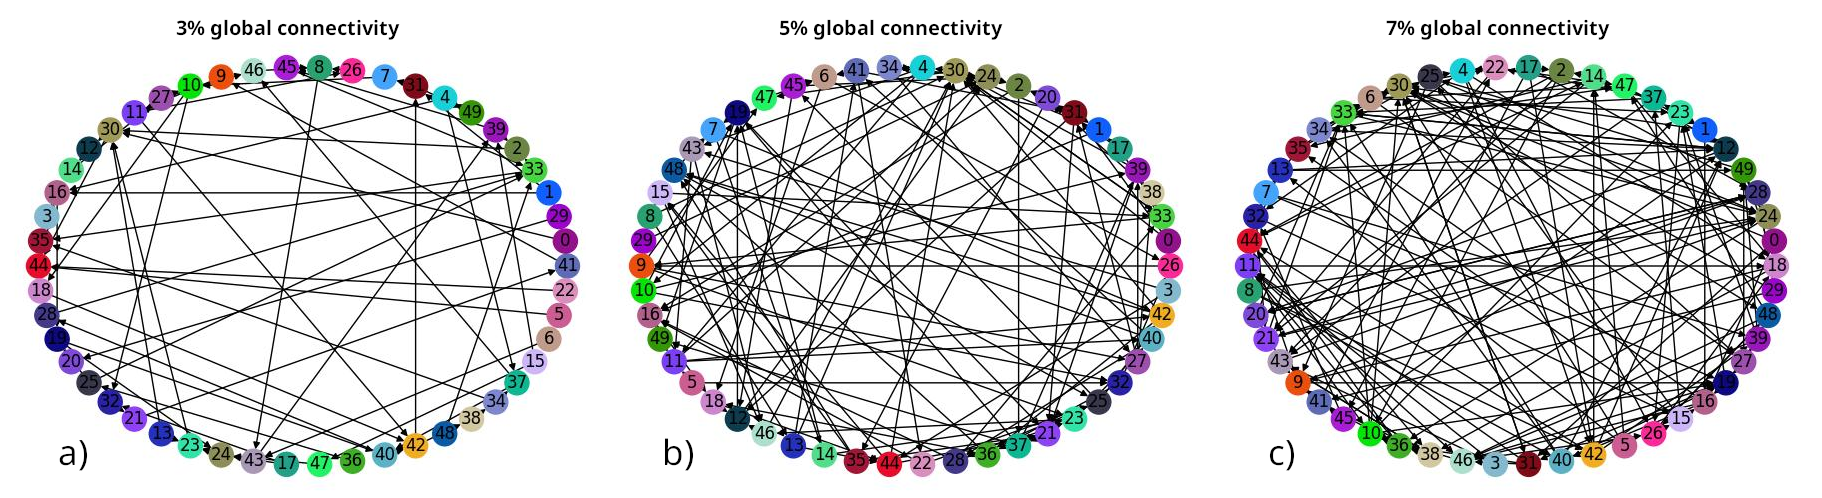
\includegraphics[width = \textwidth]{connectivity_network.png}
                \caption{Laterally Connected 50 Neuron Network}
                \label{connectivity_network}
            \end{figure*}
            
        \subsubsection{Global Connectivity Percentage}
            At this stage of the tuning process, the uniform global weights were fixed to 30. Global connectivity percentage was then tuned according to two criteria: 
            \begin{enumerate}[label=(\arabic*), leftmargin=*, rightmargin=1em, itemsep=10pt, parsep=0pt, topsep=10pt, partopsep=0pt]
                \item\label{connect1} Find the lowest value to still produce a reliable pattern.
                \item\label{connect2} Choose the lowest global connectivity percentage to still connect all neurons to form one coherent assembly. Strictly prevent any sub-networks and disconnected neurons.
            \end{enumerate}
            The global connectivity percentage was evaluated by looking at the connection graph of the 50 neuron network. Figure ~\ref{connectivity_network} shows visual examples of different connectivity percentages and their connection density.
            \begin{enumerate}[label=\alph*), labelwidth=1.5em, labelsep=1.5pt, leftmargin=1em, itemindent=0pt, rightmargin=0pt, itemsep=5pt, parsep=0pt, topsep=2pt, partopsep=0pt]
                \item\label{percent1} For a global connectivity percentage of 0.01 criterion ~\ref{connect2} was not fulfilled, where only around half of neurons formed any connection.
                \item\label{percent2} For a value of 0.03, connectivity was still too sparse, with many neurons forming only a single connection, thus not conforming to ~\ref{connect2}.
                \item\label{percent3} A percentage of 0.04 equipped some neurons with only a singular connection, which technically just about fulfilled ~\ref{connect1} and ~\ref{connect2}, but was disregarded to ensure the network would be balanced and running smoothly.
                \item\label{percent4} A percentage of 0.05 lateral connectivity in the 50 neuron network was the lowest value to reliably produce a fully connected network with each neuron forming at least two connections, while appearing relatively balanced. This value was chosen for the experiment, because it fulfilled both criteria.
            \end{enumerate}


        \subsubsection{Uniform Connectivity Weights}
            Uniform global connection weights were selected while looking at the average spike count, a reasonable measure for lateral input efficacy. Higher spike counts correlate with stronger lateral connectivity, since neurons get higher input and thus are more likely to spike. At the same time, biases are avoided for the critical dependent variables, which are synchrony and spike pattern length. To ensure that effects of lateral connectivity outweigh noise effects, the minimal requirement for the lowest universal weight value was expected to: 
            \begin{enumerate}[label=(\arabic*), leftmargin=*, rightmargin=1em, itemsep=10pt, parsep=0pt, topsep=10pt, partopsep=0pt]
                \item\label{uniform1} Increase spike count by a factor of 1.5 when compared to the spike count observed with solely noise input.
                \item\label{uniform2} From the lowest universal weight value fulfilling criterion ~\ref{uniform1}, two higher values are supposed to be selected that values show an increase in spike counnt of least 10\%.
            \end{enumerate}
            The choice to limit this experimental variable to only three values was made to stay within a reasonable scope for this project.
            
            \begin{enumerate}[label=\alph*), labelwidth=1.5em, labelsep=1.5pt, leftmargin=1em, itemindent=0pt, rightmargin=0pt, itemsep=5pt, parsep=0pt, topsep=2pt, partopsep=0pt]
                \item\label{weights1} Universal weights below 20 mV did not fulfil ~\ref{connect1}, so they were disregarded. 20 mV was set to be the lowest experimental condition.
                \item\label{weights2} For the following two values, an increase of about 15\% in average spike counts was observed with a step size of 10 mV. The values 30 mV and 40 mV, fulfilling criterion ~\ref{connect2}, were selected as the remaining two uniform weight variables.
            \end{enumerate}
            
        \subsubsection{Overview}
            The completed tuning process resulted in these parameters:

            \begin{itemize}[itemsep=0pt, topsep=2pt, leftmargin=1em, label=\tiny$\bullet$]
                \item Gaussian mean: 0.1-1.1 (step size 0.1)
                \item Gaussian SD: 0.1-1.1 (step size 0.1)
                \item Global connectivity percentage: 5\%
                \item Uniform lateral connection weights: 20, 30, 40 mV.
            \end{itemize}
            It has to be noted that a seed was set for reproducibility, thus the experiment did not need to be run more than once in the same experimental condition.

        \section{Predictions}
            In this paper I hypothesize that ~\ref{hyp1} synchrony appears with an optimal amount of non-zero noise and that ~\ref{hyp2} synchrony correlates with a shortening in pattern length due to a parallelization effect. Different noise configurations are expected to yield different results:

            \begin{figure*}[t]
                \centering
                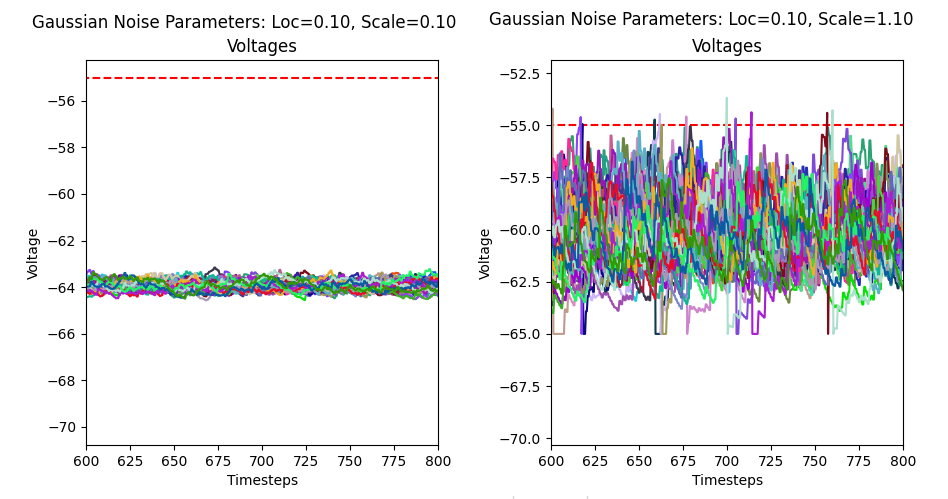
\includegraphics[width=0.8\textwidth]
                {voltage_noise_only.png}
                \caption{Voltage Recordings with Zero Interconnectivity in the 600-800ms Window}
                \label{voltage_noise_only}
            \end{figure*}
        
           \begin{enumerate}[label=\alph*), labelwidth=1.5em, labelsep=1.5pt, leftmargin=1em, itemindent=0pt, rightmargin=0pt, itemsep=5pt, parsep=0pt, topsep=2pt, partopsep=0pt]
                \item\label{pred1}Noise drawn from a Gaussian distribution with a low mean combined with low SD is predicted to lead to no spikes or few spikes. Since the voltage mean is not close enough to the firing threshold, and low SD only enables few neurons to go above, noise does not induce spikes on its own. Synchrony is not expected in cases of zero or few firings. Absolute spike pattern lengths are expected to be zero or very short in the case of few spikes, however these do not represent an actual ensemble pattern.
                \item\label{pred2}Low Gaussian mean in combination with high SD is expected to induce some spikes, which may or may not lead to ensemble patterns. Synchrony is not expected to be high with this noise configuration. Absolute spike pattern length is predicted to be long for ensemble runs and short for individual spikes which fail to activate the remaining parts of the ensemble.
                \item\label{pred3}Noise with a high mean and low SD is expected to be the optimal noise configuration for synchrony. It is predicted to activate multiple neurons at the same time, where inputs are relatiively balanced in a similarly high range for each neuron. This should lead to whole-ensemble activations with parallelized processes, which is expected to shorten pattern length compared to noise conditions where the ensemble pattern is initialized through few neurons only.
                \item\label{pred4}A high noise mean combined with a high SD is predicted to lead to diverse neuronal activations. On the one hand, high and medium noise input pushes neurons to go above the threshold, starting and continuing ensemble patterns. On the other hand, the possibility of several very low noise values may prevent certain neurons from firing when it is their turn in the pattern. This can happen even when lateral connections strongly increase the voltage of those neurons, in the case where their overall voltage was very low from receiving too little noise input. This may result in some shorter, broken patterns, but mostly longer patterns that run through the whole ensemble but fail to access efficient parallelization of spikes.
            \end{enumerate}
            Results are expected to show relatively smooth transitions between conditions.
            
		\section{Results}
            In the following section, any mentions of \textit{mean} and \textit{SD} refer to the parameters of the Gaussian ditribution utilized to draw noise values, unless explicitly stated. First, voltage and spike plots were analyzed that display observations from the 600-800 ms window of the 2000 ms trials. This time stamp was selected due to the estimate that in this window enough time had passed for noise to push sub-threshold behavior closely below the firing threshold in most conditions. While the analysis of voltage and spikes patterns was mainly based on visual plot results, the analysis of synchrony was performed analytically.

        \subsection{Voltage Analysis}
            Combinations of low mean and low SD keep membrane voltage hovering closely below the firing threshold. Voltage can be observed like a visual band, where higher means push this band towards higher overall voltage values and higher SDs widen the band to span an overall broader range of voltage values. These results are intuitive considering the function of those parameters in a Gaussian distribution. Another important observation not immediately inferred from looking at the distribution is a raise in overall voltage with increased SD but unchanged mean. This effect is caused by the clipping of below zero noise values (see Section ~\ref{sec:clipgauss}). For noise configurations where the Gaussian bell is shifted further into the negative, but then negative values are set to zero, the mean of drawn noise values turns out higher than the mean of the underlying distribution. As seen in Figure ~\ref{voltage_noise_only}, where noise was isolated from interconnected neurons (interconnections set to zero), at a noise mean of 0.1 and SD of 0.1, the voltage mean value sits at around -64 mV. In contrast, for mean 0.1 and SD 1.1 average voltage rose to about -60 mV, with gradual transition steps for in between SD values. 
            
            For higher means the effect is not visually observable, because even noise isolated from interconnections leads to frequent or continuous spiking. This results in a skewed voltage band caused by voltage resets after spiking, thus the visual bandwidth and mean of the voltage is not representative anymore.
        
        \subsection{Spike Pattern Analysis}
            Across connectivity weight conditions, low mean with low SD configurations usually lead to no spikes. Increasing either of the values results in an increase in spikes.
            
            For low means and increasing SDs, first few spikes appear, scattered across neurons (see Figure ~\ref{spikes_patterns}a)). Such spiking behavior does not lead to patterns, because spikes are too sparse. Sparseness despite strong interconnectivity can happen due to overall low noise, which fails to push voltages towards the threshold. Several neurons may receive higher noise input and spike, however, connected neurons that receive this spike as input are still likely to stay below the threshold, because their voltages were not close enough to it. Thus the ensemble breaks down after one or few spikes, preventing full patterns from emerging. As to be expected this effect varies between interconnectivity conditions: For the same noise conditions, higher interconnectivity values are likely to result in a longer spike chain, due to overall higher combined input (noise + weights).

            \noindent
            \begin{minipage}{\linewidth}
                \centering
                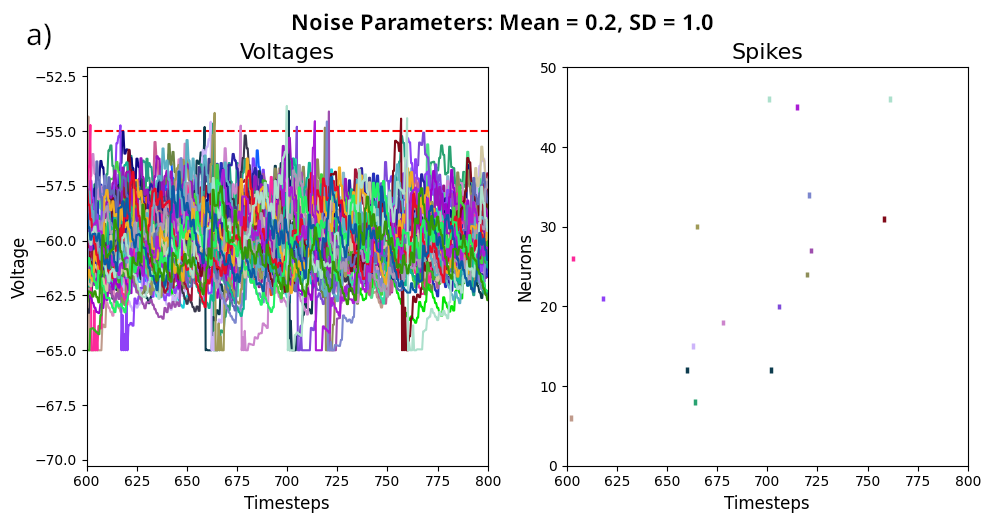
\includegraphics[width=\linewidth]{few_spikes_0.2_1.0_20mv.png}
                
                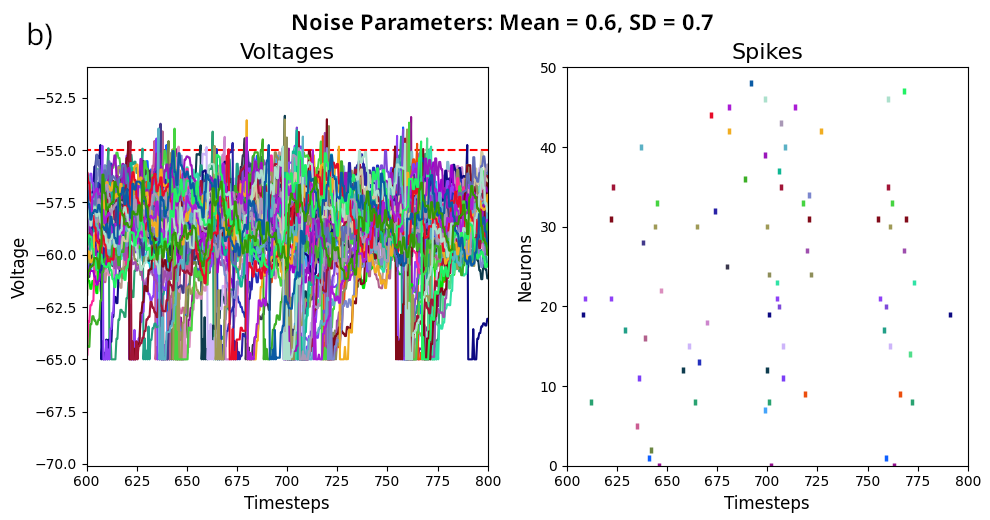
\includegraphics[width=\linewidth]{broken_patterns_0.6_0.7_20mv.png}
                
                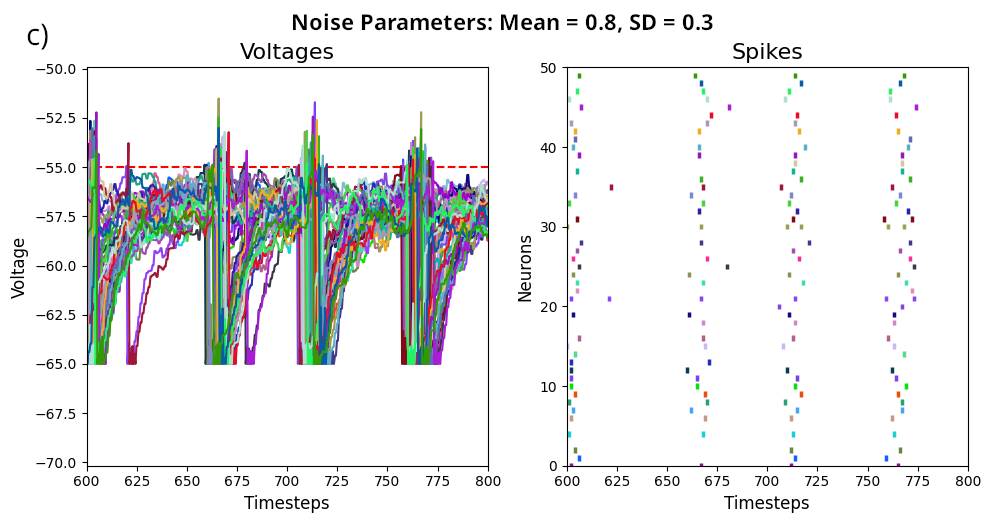
\includegraphics[width=\linewidth]{patterns_0.8_0.3_20mv.png}
                
                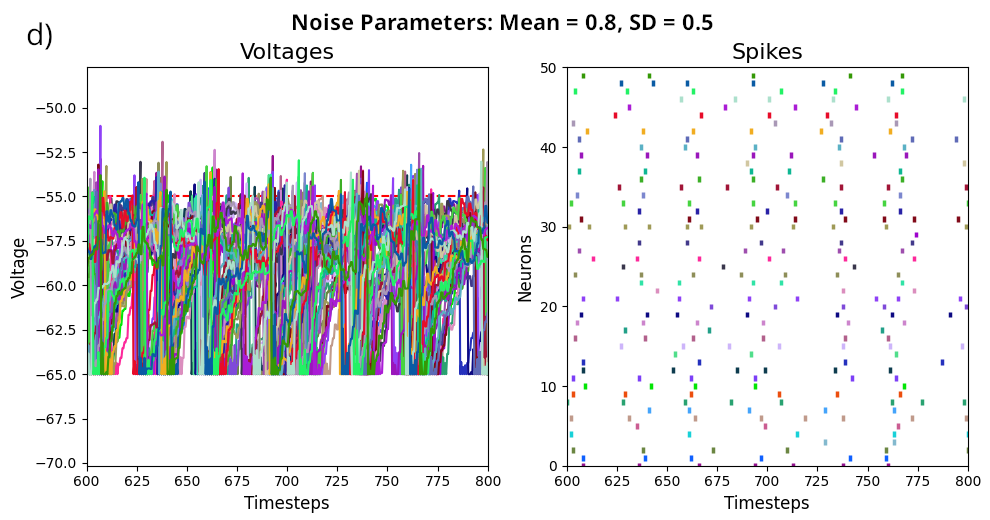
\includegraphics[width=\linewidth]{merged_patterns_0.8_0.5_20mv.png}
                \captionof{figure}{Spike Behavior in Different Noise Conditions and Corresponding Voltages for 20 mV Connectivity Weights}
                \vspace{0.5cm}
                
                \label{spikes_patterns}
            \end{minipage}

            \begin{figure*}[t]
                \centering
                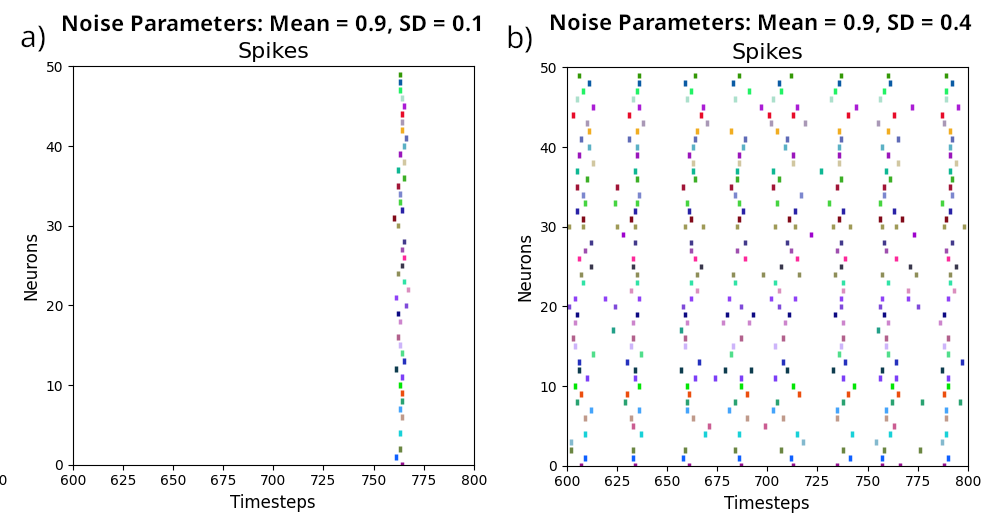
\includegraphics[width=\textwidth]{short_spikes_loc0.9_scale0.1_0.4_20mv.png}
                \caption{Visual Comparison of Spike Pattern Length in a Network with 20 mV Lateral Weights}
                \label{short_pattern}
            \end{figure*}

            For low means and increasing SDs, patterns begin to emerge visually. At first these patterns appear partially broken and not periodic, spikes still look more scattered than ordered (Figure ~\ref{spikes_patterns}b)). Transitions between \textit{no spikes \textrightarrow\ few spikes \textrightarrow\ broken patterns \textrightarrow\ periodic patterns} shift depending on the noise configuration as well as the interconnectivity weights. Especially with smaller weights, even for increasing means and arbitrary SD values, separated patterns do not emerge.
            
            For interconnectivity weights of 20 mV the first clearly distinguishable pattern appears with mean = 0.7 or mean = 0.8 (Figure ~\ref{spikes_patterns}c)),  while for a weight value of 40 mV patterns are distinguishable for the first time at a mean of 0.3. Clear patterns appear when the interconnectivity effect outweighs the noise effect. For higher interconnectivity weights, patterns are more quickly separated, because the chance for all neurons in the ensemble to be activated is higher even at lower noise amplitudes. For example, the assembly with 40 mV weights essentially gets double as much lateral input as the assembly with 20 mV connection weights. Thus, connected neurons are much more likely to fire after their preceding connections have fired, even with lower overall sub-threshold activity.
            
            Further observations can be made about the distance, i.e. the separability of patterns, once they emerge. For certain noise and connectivity configurations, patterns appear clearly separated. For 20 mV interconnectivity, the first clearly separated and full pattern appears at mean = 0.8 and SD = 0.2. This interconnectivity condition already shows emergence of patterns at lower means, but those do not appear clearly separated and may be incomplete (Figure ~\ref{spikes_patterns}b)). Once patterns have reached a point where they are clearly separated, with increasing SD they then begin to move closer together until they seem to overlap (Figure ~\ref{spikes_patterns}d)). For clearly separated patterns it appears that the higher the mean, the shorter the pattern length (see Figure ~\ref{spike_patterns}c) vs. Figure ~\ref{short_pattern}a)). These observations can be made about all interconnectivity conditions, but the onset of clearly separable patterns occurs with different noise configurations. The higher the interconnectivity weight, the earlier the onset of clearly separable patterns.

            \begin{figure*}[t]
                \centering
                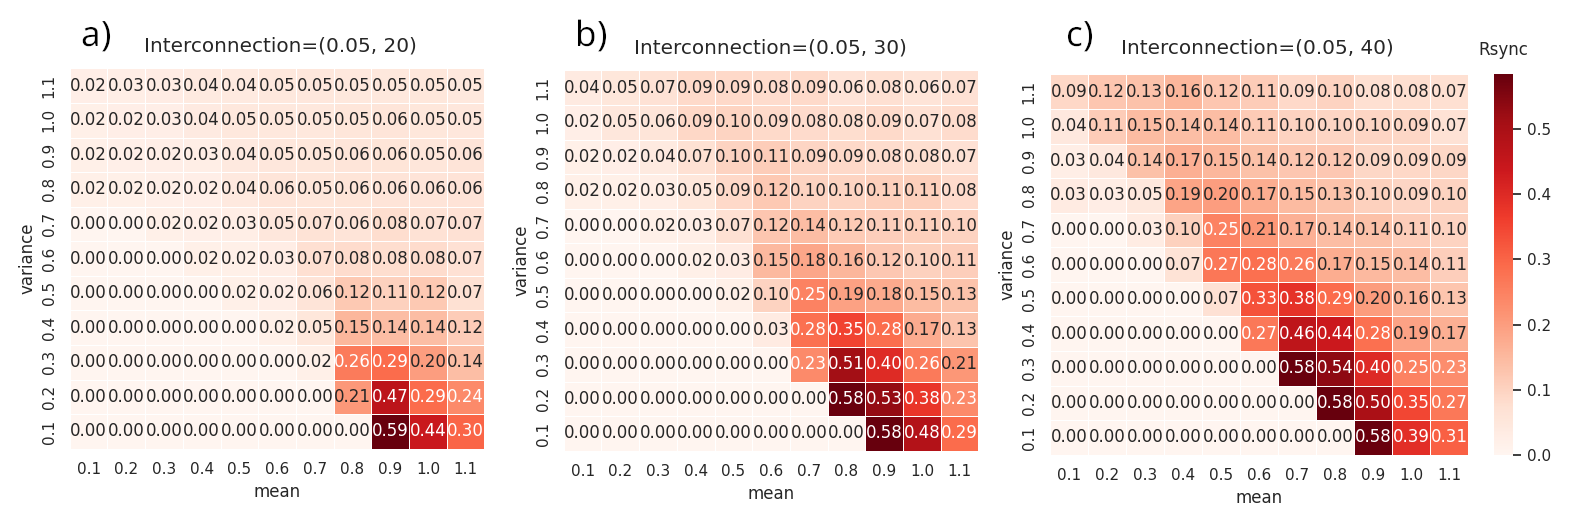
\includegraphics[width=\textwidth]{all_syncs.png}
                \caption{Rsync Results across Different Interconnectivity Conditions}
                \label{all_syncs}
            \end{figure*}
            
            
        \subsection{Synchrony Analysis}
            Next, spike behavior and synchrony were put into context: For this, spike plots were visually analyzed in the 600-800 ms window and related to the corresponding Rsync values (see Figure ~\ref{all_syncs}). For all interconnectivity conditions, zero spikes result in zero Rsync and few spikes result in very small Rsync values, usually below 0.05.

        \subsubsection{20 mV Interconnectivity}
            Increasing mean and SD leads to more spikes. For interconnectivity weights of 20 mV, a mean of 0.4 with a SD of 1.0 correlates with increased spikes. Rsync stays below 0.05, because spikes still appear very scattered without visible pattern formation. This reflects a state where effects of interconnectivity are still smaller than the noise effect. At mean = 0.7 with SD = 0.5, the 20 mV weights condition first reaches an Rsync value above 0.05. Here, visual spike trains slowly begin to separate, but reliable full ensemble runs are not detectable yet. A mean of 0.7 produces some Rsync values over 0.05, correlating with incomplete patterns, but Rsync quickly subsides again with increasing SDs: The decrease in synchrony after a peak at SD 0.6 and 0.7 correlates with incomplete spike patterns beginning to overlap.
            
            At mean = 0.8, SD = 0.2 a first onset of higher synchrony (Rsync 0.21) is recorded. This correlates with first clearly separable and complete ensemble patterns. Synchrony steadily dissipates again after a certain peak (mean 0.8, SD 0.3), at the same time as patterns have moved as closely together in time to overlap. Even once synchrony decreases with higher SD, it does not fall below Rsync of 0.05 until SD = 1.0, where patterns become inseparable. For this interconnectivity condition, a global peak of synchrony (Rsync 0.59) is reached at mean = 0.9 and SD = 0.1, with the visually shortest patterns for this mean (Figure ~\ref{short_pattern}a) and b)).

            With increasing SD, patterns widen and move closer together. At a mean = 0.9, from SD = 0.3 to SD = 0.4, synchrony drops to a lower value, from Rsync 0.29 to 0.14. This Rsync drop correlates with drastically shrinking separation intervals. Increasing SDs for same mean (0.9) show the beginning of overlapping patterns. At mean = 1.0 and SD = 0.1, synchrony is still comparably high (Rsync 0.44), but lower (Rsync 0.59) than for the previous mean (0.9) at the same SD value (0.1). This decreased synchrony is reflected in shorter separation intervals compared to the previous mean (0.9) condition. Since 0.1 is the lowest possible SD value in this experiment, it can be assumed that synchrony would peak at even smaller SD values, but it is unclear whether smaller SD values would be reasonably applicable.
            
            For the last mean (1.1), synchrony begins high again (Rsync 0.3), with the peak possibly out of range. Here, patterns appear separable and very short, but with an already small separation interval. Because of these short separation intervals, patterns quickly begin to merge as SD increases.
        
        \subsubsection{30 mV Interconnectivity}
            For interconnectivity weights of 30 mV, synchrony and spike behavior look different to 20 mV weights in noise conditions that produce more than a few scattered spikes. Here, rough, incoherent patterns can already reach Rsync values a little over 0.05, which can be observed for mean = 0.3, SD \ensuremath{\geq} 1.0 and mean = 0.4, SD \ensuremath{\geq} 0.9. For means \ensuremath{\geq} 0.5, synchrony appears at a certain SD level and then decreases again after a singular peak. The higher the mean, the lower the SD value needs to be to exhibit synchrony: for mean = 0.6, onset happens at SD = 0.5, peak at SD = 0.7 with an Rsync value of 0.15, and it subsides gradually from SD = 0.7 onwards. For mean = 0.8, the onset of higher synchrony, also marking the peak, already appears at SD = 0.2. The Rsync peak for this mean is nearly quadrupled (0.58) compared to the peak of mean = 0.6 (Rsync = 0.15). Synchrony at mean = 0.8 subsides from SD = 0.3 onwards, with stronger synchrony decreases between SD steps compared to previous means. With this trend of earlier synchrony onset, it should be considered that the peaks for means \textgreater 0.9 may fall out of the experiment's recording range. This would be in line with the observation that means \textgreater 0.9 have shrinked peak values at the lowest possible SD value (0.1).
            
            Overall, Rsync peaks in the 30 mV weights condition correlate with the most separable of full patterns, and decreases of synchrony at higher SD values correlate with the degree of pattern overlap. Higher means result in overall stronger synchrony and shorter full patterns, as long as separability is maintained. This effect can be observed when looking at the global peak in synchrony, which correlates with very short patterns and long separation intervals. Decreases in synchrony at higher SDs then correlate with smaller separation intervals, where pattern length stays consistent. For mean = 1.1, SD = 0.1, patterns are very short and still separable, with an Rsync value of 0.29. Synchrony is only half as strong as the global maximum despite its short intervals, presumably due to the weakened separability effect, despite clear visual separation.
            
        \subsubsection{40 mV Interconnectivity}
            For the 40 mV lateral weight condition, synchrony for zero spikes and few scattered spikes behaves the same as with the other interconnectivity conditions. Zero spikes result in Rsync = 0 and for very few spikes Rsync stays below 0.05. In this interconnectivity condition, the onset of synchrony happens even earlier. A mean of 0.2 with SD = 1.0 already shows separable yet broken patterns, with a first Rsync value over 0.05. For comparison: with 20 mV lateral weights, first Rsync \textgreater 0.05 is reached at mean = 0.6, SD = 0.8. With 40 mV, the interconnectivity effect quickly overpowers the noise effect. Observed patterns are more variable in length and separation intervals for low mean, high SD combinations, than for higher means.
            
            At mean = 0.5, SD = 0.6, Rsync first reaches a value over 0.2, a comparably high value, with more stable pattern and separation interval lengths. Synchrony again subsides where patterns begin to merge. The global synchrony peak for 40 mV weights is recorded at mean = 0.7 and SD = 0.3, but it is notable that this global peak happens three times in total, from mean = 0.7 to mean = 0.9. With each increasing step of means, the SD value for the same Rsync is one lower than for the previous. For all three global peaks synchrony subsides from the next SD value onwards, where an earlier decrease also correlates with earlier fading, with comparable step sizes. Here again, higher synchrony correlates with increased separation interval length and shortness of patterns. This can roughly be estimated from the visual spike patterns in the 600-800ms window: The results in Table ~\ref{table1} show that a correlation of increased synchrony with shortness of patterns and separability is to be expected. So far it is inconclusive whether one of the two factors is a stronger or the main predictor for synchrony. To compare the effects of separability and pattern length, specific examples were selected that were able to compare two cases:
            \begin{enumerate}[label=(\arabic*), leftmargin=*, rightmargin=1em, itemsep=10pt, parsep=0pt, topsep=10pt, partopsep=0pt]
                \item\label{diffsep} Similar pattern lengths but different separability intervals (mean 0.7, SD 0.3, 40 mV, higher separability; mean 0.8, SD 0.3, 40 mV, lower separability).
                \item\label{diffpattern} Different pattern lengths but similar separability intervals (mean 0.5, SD 0.7, 40 mV, longer patterns; mean 0.8, SD 0.3, 40 mV, shorter patterns).
            \end{enumerate}
            Those two comparisons showed that:
            \begin{enumerate}[label=(\arabic*), leftmargin=*, rightmargin=1em, itemsep=10pt, parsep=0pt, topsep=10pt, partopsep=0pt]
                \item[\ref{diffsep}]If pattern length was similar, synchrony was observed to be higher for intervals that are further separated in time (Rsync 0.58) than for patterns with lower separability (Rsync 0.54).
                \item[\ref{diffpattern}] For similar separability intervals, shorter patterns showed higher synchrony (Rsync 0.54) than longer patterns (Rsync 0.25).
            \end{enumerate}
            It has to be noted that these observations are very sparse, because the experiment was aimed at a different purpose. Further research is needed to investigate the relationship of pattern length and separability as a predictor for synchrony.

        \end{multicols}
        
            \begin{table*}[h]
                \centering
                \caption{Pattern and Separation Intervals with 40 mV weights}
                \label{table1}
                
                \begin{tabular}{*5l}    \toprule
                    \textbf{Gaussian Mean} & \textbf{0.7} & \textbf{0.8} & \textbf{0.9} \\\midrule
                    \textbf{Gaussian SD} & \textbf{0.3} & \textbf{0.2} & \textbf{0.1} \\ 
                    Rsync & 0.58 & 0.58 & 0.58\\
                    Separation Intervals & \textgreater 150ms & \textgreater 150ms & \textgreater 150ms\\
                    Pattern Length & $\sim$ 5-8ms & $\sim$ 5-8ms & $\sim$ 5-8ms\\\midrule
                    \textbf{Gaussian SD} & \textbf{0.4} & \textbf{0.3} & \textbf{0.2} \\ 
                    Rsync & 0.46 & 0.54 & 0.50\\
                    Separation Intervals & $\sim$ 15-70ms   & $\sim$ 20-75ms & $\sim$ 15-50ms\\
                    Pattern Length & $\sim$ 8ms & $\sim$ 8ms & $\sim$ 5-8ms\\\bottomrule
                    \hline
                \end{tabular}
            \end{table*}

        \begin{multicols}{2}
            
            Comparing the global peaks of the 30 mV with the 40 mV weight condition, for the former, the same value (Rsync 0.58) is first recorded at mean = 0.8, SD = 0.2, whereas for the latter it already appears with mean = 0.7, SD = 0.3.  While with 30 mV weights this value is recorded twice under selected noise conditions, with 40 mV weights this value is recorded three times, most probably due to an earlier onset of synchrony. With increasing means this peak is consistently observed at smaller SD values. This would predict it to fall out of range from mean = 1.0 onwards, after it was observed for the smallest SD value (0.1) for a mean of 0.9. This assumption can confirmed for both the 30 mV and 40 mV interconnectivity condition.
            
        \subsection{Average Pattern Length Analysis}
            While conducting the experiment, I also recorded an average pattern length. However, the results do not reflect visually estimated pattern lengths consistently well under different noise conditions. This was likely due to the experimental nature of the recording method, as well as the strong variations in pattern lengths for some conditions. For completeness, results of the experimental pattern length measure are presented as well, although they were not used to draw definite conclusions.
            
            The results of this measure look similar across all interconnectivity conditions. For low means and SDs no pattern lengths are recorded, which correlates with the absence of spikes. With low means but higher SDs, average pattern length appears to lie between 1 and 3 ms. This correlates with the observation that interconnections struggle to continue the pattern due to low overall low voltage. With increasing means, lower SD values can already result in spikes and thus average pattern length is recorded here as well. A trend of shorter average pattern length correlating with higher synchrony can be observed, where combinations of high means and low SDs yield best synchrony results and comparably small average pattern lengths of 6 to 8 ms. With increasing SDs at higher means, average pattern length increases, with values of 10 to 20 ms. This trend is disrupted by some outliers, such as 18 ms at 20 mV interconnectivity weights at mean = 0.8, SD = 0.2, despite high synchrony (Rsync 0.21). These outliers where synchrony is very high and pattern length is not as short as expected, can be attributed to the experimental nature of the average pattern length measure, as well as the way the Rsync measure works. Rsync does not only take the degree of spike parallelization into account, but also separability, which can be seen in the length of separation intervals. Those outlier values do not have the shortest patterns, but still show high Rsync, because separation intervals are very long, increasing the separability effect.


        \section{Discussion}
        \subsection{Interpretation of Findings}
			The present paper has revealed that synchrony can emerge in a recurrent spiking neural network receiving an optimal non-zero amount of Gaussian noise input. What makes those noise parameters optimal depends on the lateral connectivity of the neuron ensemble. With lateral connectivity strong enough to connect a whole network without creating gaps or subnetworks, synchrony onset depends on the strength of connections between neurons. In a network with stronger interconnections, the onset of synchrony appears at lower noise input and the network displays higher overall Rsync values, compared to a network with weaker interconnections.
            
            A general trend for the Gaussian noise parameter configuration points towards a combination of high mean and low SD. In order to reach optimal Gaussian noise conditions inducing synchrony, a high chance for multiple neurons to spike in parallel has to be achieved. Combinations of low mean and low SD fail to spike enough neurons, because sub-threshold behavior stays too far away from the firing threshold, thus no spikes are elicited without external input. If the SD is increased, despite a low mean parameter, some neurons may be pushed close enough to the threshold due to occasional higher noise values. However, since the voltage of most neurons is still too far below the threshold, most lateral connections will not be strong enough to cause a spiking chain reaction, failing to activate the whole ensemble pattern. If instead SD is kept low but the mean is increased, the voltage of more or most neurons will closely hover below the threshold, which then makes it possible for even small variant noise inputs to push neurons over the threshold. As soon as one neuron is activated, the interconnectivity effect is strong enough to activate the whole ensemble, creating a characteristic spike pattern representing the structure of this specific network. Depending on the mean value, one of the lowest SD values induces the highest synchrony, due to the activation of multiple neurons at the same time. Instead of running through the ensemble pattern from beginning to end, multiple parts of the pattern are activated at the same time, thus parallelizing processes. This way, the time it takes to run through the whole ensemble is shortened, decreasing the overall length of the pattern without compromising the information conveyed. In conclusion, Gaussian noise with lower SD and higher mean values comprises the most optimal noise for synchrony induction.
            
            When SD is increased from this optimal noise setup, synchrony slowly dissipates again, until the noise effect begins to override the interconnectivity effect. Rsync values decrease due to reduced information distinction, which is caused by the patterns moving closer together. This reduction in separation interval length is caused by an increased probability for higher than average noise values, inducing more frequent ensemble runthroughs. When SD is set even higher, patterns are pushed even closer together in time until they merge and synchrony dissipates. Under such noise conditions neurons still fire simultaneously, but the amount of firings begin to overlap so much that they lose their ability to discern information, and hence the coding quality of synchrony gets lost in information overload. \textcite[p. 55]{G} calls this kind of issue a "superposition problem".
            
        \subsection {Implications}
            The findings in this study pose important implications for research on synchrony as a coding mechanism. Firstly, the induction of synchrony in a laterally connected neural network through noise shows the internal coordination capabilities of simple neural network feedback loops. It opens up the possibility for synchrony as an internal neuronal mechanism occurring with or without external input. In addition, this experiment 
            highlights that biological neural networks, which are exposed to high amounts of noise, may not just reliably work in spite of, but because of said noise. The findings in this study are in line with the results of \textcite{P} and \textcite{Q}, who found that an optimal amount of non-zero noise promotes the emergence of synchrony. From these results it can be assumed that the brain is capable of much richer information processing than previously predicted and that not all present noise is simply filtered out.
            
            Secondly, the observed shortening of patterns demonstrates the capability of spike synchrony to increase information coding efficiency by parallelizing processes. Synchrony thus shows strong potential as a coding mechanism because of its high efficiency and capability to encode distributed information, as has been shown in other literature \cite{R, L}. It is expected to operate as a complementary mechanism to rate code \cite{L, G}.

            The results in this study could inspire future research to further investigate the underlying mechanism of synchrony emerging from noise. Promising insights may be derived from dynamical systems theory, where theories of the brain modeled as a dynamical system could reveal that neural pocessing may rely on noise for the emergence of synchrony \cite{Y}. Advancing theories about the emergence of synchrony through noise could then support the development of experiments to test whether this mechanism of noise-induced synchrony can actually be observed in biological neuronal networks.

        \subsection {Limitations}
            Because of the simplicity of this study, further research is needed on more biologically plausible models to confirm the shortening of patterns linked to increased synchrony. The model in this study was constructed to resemble a biological system as best as possible, however, due to the scope of the project, some variables were strongly simplified. One of these simplified variables are interconnection weights, which were set to a uniform weight value for each neuron in the network. In future experiments such lateral weight values should be drawn from a distribution to mimic the variability in connection strengths that biological neurons display \cite{J}. Furthermore, the network should be implemented with a learning algorithm and assigned a task, to provide evidence that pattern shortening correlating with synchrony is not solely produced under artificial circumstances, but also appears in actual applications of the network. A good example of models studying synchrony in task application are \textcite{L} and \textcite{M}, both investigated synchrony as a measure of familiarity. This type of task is particularly interesting in combination with a Spike-Time-Dependent Plasticity (STDP) learning algorithm, as it utilizes a form of Hebbian learning, a mechanism where synchrony is harnessed for Long-Term Potentiation (LTP) and Long-Term Depression (LTD) \cite{A, L}.
            
            Along with applied models of synchrony, more experimental evidence needs to be gathered to prove that the efficiency of synchrony code is actually what is harnessed by biological systems. While synchrony has previously been found in biological neural networks, further research needs to distinguish which functions it serves biologically, compared to the potential functions observed in theoretical models \cite{L, M}.
            
            It also needs to be further investigated whether separation intervals or pattern shrinkage are the stronger predictor of synchrony. Since the experiments in this paper were focused on investigating the effect of synchrony on pattern length, the results did not serve to sufficiently analyze interactions separation interval length. It therefore cannot be fully concluded that pattern shrinkage stands in stronger correlation with synchrony than separation interval length.
            
            A further limitation of this study poses the experimental nature of the pattern length measuring techniques. Average Pattern Length was measured in a very simplified way, capturing the time window where at least one spike was recorded across the entire network per time step. However, this method does not check whether the spike sequence was caused by an actual connectivity pattern and if exactly one full pattern was counted. Further pattern length analysis was carried out on spike train visualizations, which only allows for approximations instead of precise measurements. Different measures need to be developed to determine pattern length more accurately.


        \section{Conclusion}
            This study has shown that synchrony is a process where distributed neural signals are coordinated. With increased synchrony, more signals can be processed at the same time, which results in shorter overall processing time. Furthermore, the experiment provides an example that synchrony can emerge from an optimal amount of non-zero noise without external input, in a laterally connected neural network. Such optimal noise promotes the separation and compression of spike patterns, whereas less optimal noise fails to activate the whole pattern or moves patterns too closely together, where information gets lost due to overlap.
            
            From these results it can be assumed that synchrony is a viable coding scheme in neurons and that it can be harnessed to efficiently process information that other coding schemes struggle to interpret. This applies specifically to distributed and time-sensitive information, which loses its informative value when converted to the more commonly investigated rate code. It was also displayed that synchrony code is much more efficient in propagating information, because of its parallelization capabilities.
            
            It can be expected that synchrony code will become increasingly important in future research, because of its multiple advantages over rate code for certain tasks. Its ability to coordinate neural networks on a multi-cell basis is a crucial novel research area for understanding how complex thoughts as we experience them are built from the interplay of neuronal signals on the basis of small units.

		
		\section{Methods}
		\subsection{Spiking Model}\label{sec:LIF}
            For the spiking model, the Leaky Integrate-and-Fire (LIF) neuron was chosen, a state-of-the-art neuron model for spiking neural networks \cite{A}. This model is inspired by electronic principles and allow to take membrane time constant, firing threshold and refractory period into account for the integration. It provides the advantage of simulating a logarithmic external stimulus to neural output relationship, which is observed in biological neurons \cite{E}. The formula used in this paper was taken from \textcite{L}:
            \begin{gather}\tau_{m}\frac{dV_{i}}{dt}=-(V_{i}-E_{L})+RI_{i}(t)\end{gather} where $dV$ is the membrane potential update with a step size of $dt$ in ms, and with the time constant $\tau$ in ms. $V$ concerns the current voltage of the neuron, $E_{L}$ describes the resting potential and $RI_{i}(t)$ are the incoming synaptic currents. $R$ represents a finite leak resistance of the cell membrane \cite{L, ZN}.
            
        \subsection{Synchrony Measure}\label{sec:sync}
            To record synchrony, i.e. the degree to which neurons fire together, the Rsync measure was selected. The advantage of Rsync over other synchrony measures is its scalability to any higher neuron population sizes. It works by averaging the population mean variance by the average individual neuron variance. Through this mechanism, independently firing neurons push Rsync towards 0, whereas synchronous firing averages Rsync towards 1 \cite{L}. The Rsync formula was taken over from \textcite{L}: \begin{gather}R_{sync}(P, T) = \frac{\hat{\text{Var}}[\langle A_{i}(t) \rangle_{i \in P}]_{t \in T}}{\langle \hat{\text{Var}}[A_{i}(t)]_{t \in T} \rangle_{i \in P}}\end{gather} $P$ represents the encoded pattern of the neuron population and $T$ the ms time interval. $A_{i}$ describes an activation trace of a neuron $i$ that is part of the population $P$. Activation traces become more similar with increasing synchrony, and would all be identical for perfect synchrony \cite{L}.

            \begin{figure*}[t]
                \centering
                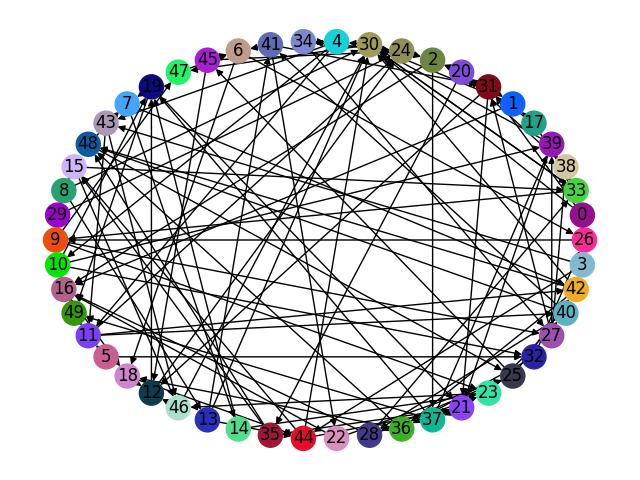
\includegraphics[width=0.5\textwidth]{model_connectivity.jpg}
                \caption{Laterally Connected 50 Neuron Network}
                \label{network}
            \end{figure*}
            
        \subsection{Average Spike Pattern Length}\label{sec:patternlen}
            Average Spike Pattern Length is an experimental measure developed for this paper, with the intention to make pattern length analysis comparable. For this method a total spike count across the whole neuron population was counted and each time step with at least one spike count was recorded as part of the pattern. Every coherent sequence of time steps with at least one spike was summed together as one pattern to yield the amount of time steps per pattern, i.e. the pattern length. Any amount of empty time steps were defined as separation intervals, but were not recorded in length. Of the recorded pattern lengths a mean was taken per experimental condition, resulting in the Average Pattern Length Value. The choice to count even singular spikes as part of patterns, versus selecting a threshold of at least a few multiple firings, was made under the assumption that one spike would already be of value to the pattern. Due to the strong interconnectivity of the network, it was expected that most singular spikes would activate further neurons in the following time step. From that it was concluded that singular spikes were more likely to be informative than not.
            
            It has to be noted that this measure is very limited in its informative value, because depending on the noise and interconnectivity condition, pattern length was more similar or more variable. It served to point towards a trend, but to ensure detailed and robust results, visual pattern analysis was considered more informative over the Average Pattern Length Value.

        \subsection{Model Connectivity}
            To fit the scope of the experiment, a laterally connected 50 neuron network was set up with a 5\% connectivity value, which translates to each individual neuron in the network being connected to approximately 5\% of other neurons. Connectivity was set up semi-randomly, where a random draw was followed by a rule for an upper limit of incoming connections, to ensure balanced lateral connectivity. Weights between neurons were set to a uniform value for the whole network, only differing with interconnectivity conditions. The network shown in Figure ~\ref{network} was used for all experimental runs.
    
    \section {Code Availability}
        The code of the experiment and the experimental plots are available at \url{https://github.com/Mini11e/spiky\_project.git}.
    
    \section{Declaration of AI Use}
        AI was explicitly not used for writing in any circumstance, except within browser searches for synonyms and words. For Google searches the AI assistant answers were occasionally taken as general input, but never used as a credible sources for any content written in this paper. For some \LaTeX\ code issues, AI was harnessed to debug or adapt code to improve formatting. In the beginning of the code building process of the experiment, AI was used once to create a small and simplistic model to gain an overview of what a model may be structured like. This model was completely discarded from the actual experiment, but the file can still be found in the codebase under \verb|/TEST_model_first_version_AI|.

    
    \printbibliography
    \end{multicols}

    \newpage
    \section{Appendix}

        \begin{figure}[H]
            \centering
            \caption{Rsync, Average Spike Count, Average ISI and Average Pattern Length Recordings for 20 mV Interconnectivity Weights}
            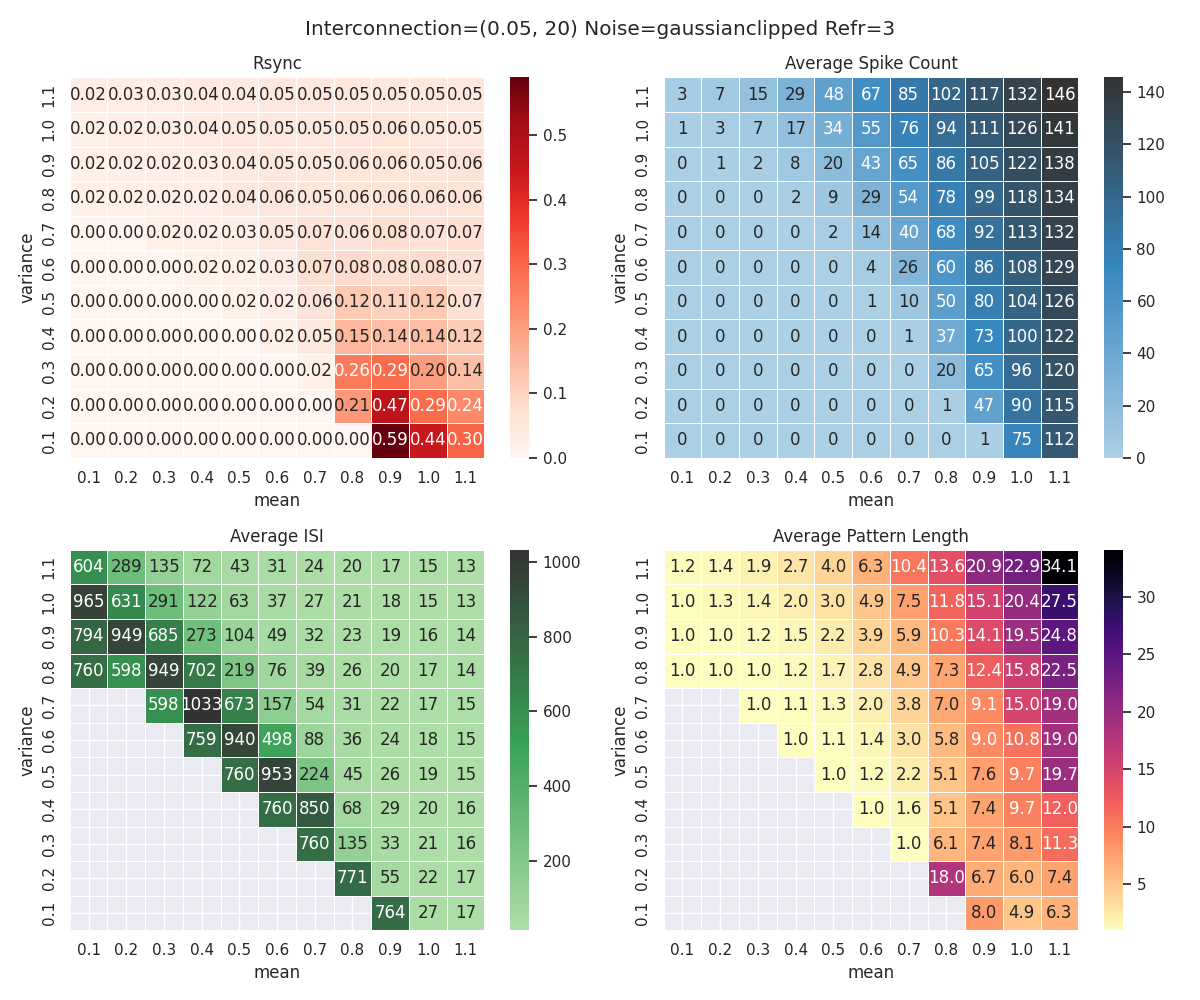
\includegraphics[width=\textwidth]{heatmaps_20mv.png}
            \label{appendix1}
        \end{figure}

        \begin{figure}[H]
            \centering
            \caption{Rsync, Average Spike Count, Average ISI and Average Pattern Length Recordings for 20 mV Interconnectivity Weights}
            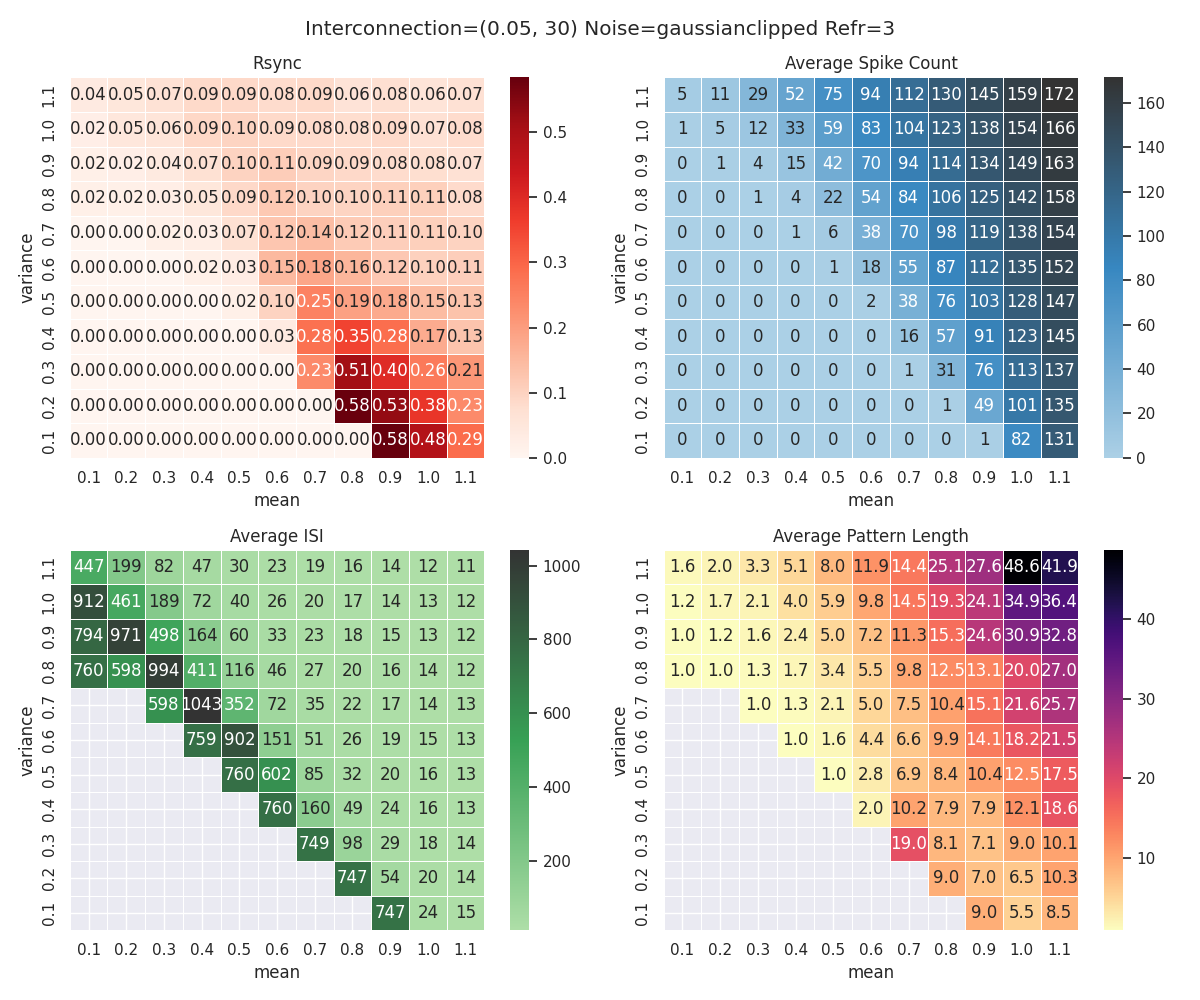
\includegraphics[width=\textwidth]{heatmaps_30mv.png}
            \label{appendix2}
        \end{figure}

        \begin{figure}[H]
            \centering
            \caption{Rsync, Average Spike Count, Average ISI and Average Pattern Length Recordings for 20 mV Interconnectivity Weights}
            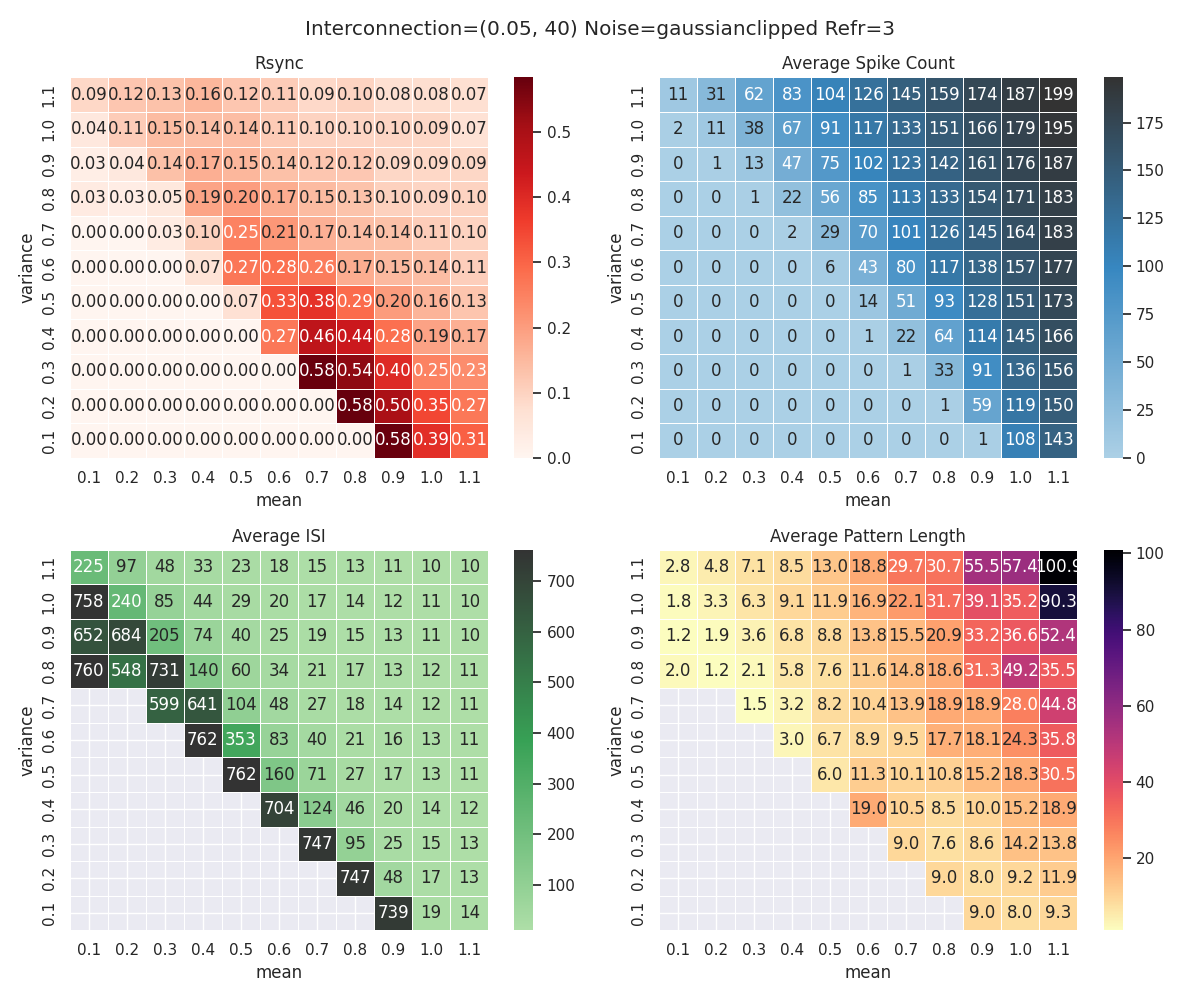
\includegraphics[width=\textwidth]{heatmaps_40mv.png}
            \label{appendix3}
        \end{figure}


	
    
\end{document}